\subsection{Environment ablations: when does learning add value?}\label{sec:ablation}
To separate the contributions of the environment's components, we retrained AA-DQN (five seeds) in four variants and re-tuned every heuristic for each variant. Table~\ref{tab:ablation} and Fig.~\ref{fig:ablation} report the difference between AA-DQN and the best heuristic \emph{within} each variant. This avoids comparing returns across variants with different reward scales.

\emph{Observation quality is the main bottleneck.} When attention and fatigue are observed without noise, AA-DQN improves to \ablNoObsNoiseRet{} and exceeds the best heuristic (\ablNoObsNoiseBest, \ablNoObsNoiseBestRet) by $+\ablNoObsNoiseDiff$ ([\ablNoObsNoiseLo, \ablNoObsNoiseHi]) in return and $+\ablNoObsNoiseDiffOnPP$ percentage points in on-time rate. Its mean fatigue also falls, from \aaFatigue{} in the nominal setting to \ablNoObsNoiseFatigue. The heuristics do not benefit from perfect information at all: the best threshold rule is no better than with noisy observations, because a fixed threshold cannot use precise state information beyond the threshold crossing. Learned policies thus have a structural advantage that grows with sensor quality, while the advantage of hand-crafted rules does not.

\emph{The circadian process is not what the agent exploits relative to rules.} Without the circadian term, AA-DQN and the best rule are tied in return ($+\ablNoCircadianDiff$, [\ablNoCircadianLo, \ablNoCircadianHi]), and AA-DQN keeps a $+\ablNoCircadianDiffOnPP$ pp on-time advantage. This is the same pattern as in the full model, so the agent's behaviour around the post-lunch dip (Section~\ref{sec:behaviour}) is an adaptation to the dynamics rather than the source of an advantage over the threshold rules.

\emph{The cognitive reward terms are not responsible for the result.} Trained with a task-only reward ($\lambda=\mu=0$), AA-DQN still matches the best rule in return ($\ablTaskRewardOnlyDiff$, [\ablTaskRewardOnlyLo, \ablTaskRewardOnlyHi]) and still rests in \parZeroBrkPct\% of slots (Table~\ref{tab:pareto}), because rest pays off through productivity alone. The agent's on-time advantage disappears in this variant ($\ablTaskRewardOnlyDiffOnPP$ pp), which indicates that the attention term shapes \emph{how} it trades completions against cognitive load.

\emph{Learning also helps without cognitive dynamics.} In the static-capacity variant, in which rest has no value, AA-DQN beats the best rule (SPT) by $+\ablNoCognitionDiff$ ([\ablNoCognitionLo, \ablNoCognitionHi]) and $+\ablNoCognitionDiffOnPP$ pp. Under overload, combining urgency (EDF) with processing time (SPT) depending on the state of the queue is better than either rule alone, a well-known property of composite dispatching \cite{haupt1989,luo2020}. This result does \emph{not} support the claim, made in an earlier version of this work, that reinforcement learning helps only when cognition is modelled. What cognitive dynamics change is the size of the stakes: in the full model, state-aware policies exceed the capacity-agnostic rules by 4--8 return units (Table~\ref{tab:main}), versus 1--3 units in the static model.

\begin{table}[!htbp]
\centering
\caption{Environment ablations. AA-DQN (five seeds) versus the best re-tuned heuristic within each variant; differences are paired over 500 test days with 95\% bootstrap CIs (on-time in percentage points).}
\label{tab:ablation}
\small
\resizebox{\textwidth}{!}{\begin{tabular}{lcccccc}
\toprule
Environment variant & AA-DQN return & Best heuristic (return) & $\Delta$ return [95\% CI] & AA-DQN on-time & Best heuristic (on-time) & $\Delta$ on-time [95\% CI] \\
\midrule
Full model & 12.19 $\pm$ 0.27 & EDF-Periodic (11.41) & +0.77 [+0.58, +0.96] & 0.726 & EDF-Periodic (0.660) & +0.066 [+0.057, +0.075] \\
\bottomrule
\end{tabular}}
\end{table}

\begin{figure}[!htbp]
\centering
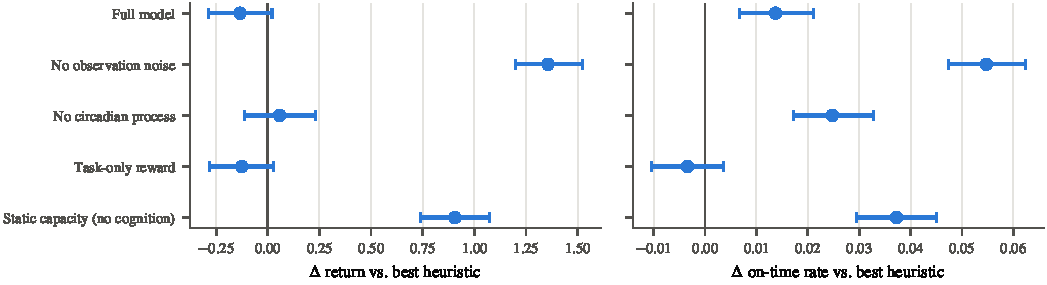
\includegraphics[width=\textwidth]{figures/fig_ablations.pdf}
\caption{Difference between AA-DQN and the best heuristic within each environment variant (95\% CIs). Positive values favour AA-DQN.}
\label{fig:ablation}
\end{figure}

\subsection{Productivity--fatigue trade-off}\label{sec:pareto}
The fatigue weight $\lambda$ (with $\mu=\lambda/2$) controls how much the agent values the worker's state. Figure~\ref{fig:pareto} and Table~\ref{tab:pareto} show the policies obtained for $\lambda\in\{0,0.05,0.1,0.2,0.4\}$. Increasing $\lambda$ lowers mean fatigue monotonically, from \parZeroFat{} to \parZeropFourFat, by raising the break share from \parZeroBrkPct\% to \parZeropFourBrkPct\%. Over most of this range it does \emph{not} reduce productivity. The on-time rate rises from \parZeroOnPct\% ($\lambda=0$) to \parZeropTwoOnPct\% ($\lambda=0.2$), and is still \parZeropFourOnPct\% at $\lambda=0.4$. At $\lambda=0.4$, AA-DQN keeps the worker \emph{less} fatigued than any of the tuned heuristics (Fig.~\ref{fig:pareto}) while completing more tasks on time than the best of them (\bestHeurOnTimePct\%). Moderate concern for the worker's state is therefore not a cost to productivity but a means to it, which echoes empirical findings on rest breaks \cite{henning1997,dababneh2001,albulescu2022}. The fatigue penalty of the nominal agent noted in Section~\ref{sec:main} is a consequence of the chosen weight, not of the method.

\begin{figure}[!htbp]
\centering
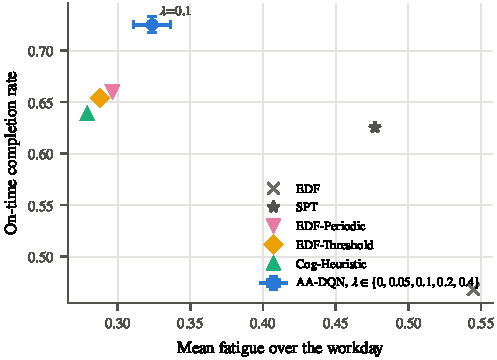
\includegraphics[width=0.62\textwidth]{figures/fig_pareto.pdf}
\caption{Productivity--fatigue trade-off. AA-DQN trained with different fatigue weights $\lambda$ (three seeds each; error bars: s.d.) versus the tuned heuristics.}
\label{fig:pareto}
\end{figure}

\begin{table}[!htbp]
\centering
\caption{Effect of the reward weight $\lambda$ on AA-DQN (mean $\pm$ s.d.\ over three seeds; 500 test days).}
\label{tab:pareto}
\small
\begin{tabular}{cccccc}
\toprule
$\lambda$ ($\mu=\lambda/2$) & On-time rate & Mean fatigue & High-fatigue exposure & Break share \\
\midrule
0.1 & 0.725 $\pm$ 0.008 & 0.324 $\pm$ 0.013 & 0.000 & 0.163 \\
\bottomrule
\end{tabular}
\end{table}

\subsection{Component analysis}\label{sec:component}
Table~\ref{tab:component} isolates the components of AA-DQN (three seeds each, except for the ten-seed configurations). \emph{Memory is essential.} Removing the observation history ($k=1$) reduces the return from \compAADQNRet{} to \compAADQNNoHistRet, close to the vanilla DQN, and a two-step history recovers only part of the loss (\compAADQNKTwoRet). An eight-step history performs at least as well as $k=4$ (\compAADQNKEightRet). A GRU encoder over an eight-step window performs similarly (\compAADQNGRURet), so the benefit comes from the length of the memory rather than from recurrence per se. In contrast, Double Q-learning and the dueling head have small effects within seed variability (\compAADQNNoDoubleRet{} and \compAADQNNoDuelingRet{} without them). This indicates that the partial observability of the cognitive state, not value over-estimation, is the main difficulty of the problem.

\emph{A smaller action space learns better.} The agent restricted to the intensity actions \{\textsc{easy}, \textsc{hard}, \textsc{break}\} achieved the highest return of all configurations in the three-seed study (\compAADQNThreeactRet). Because this variant was not our pre-specified primary method, we did not promote it on the basis of three seeds. Instead, we re-evaluated it with the full ten-seed protocol as a secondary analysis (Section~\ref{sec:secondary}). The result is plausible in hindsight. With the shortest-task feature in the observation, choosing an easy (typically short) task already captures much of the benefit of SPT, while the larger hybrid action space slows exploration and credit assignment.

\begin{table}[!htbp]
\centering
\caption{Component and sensitivity analysis (mean $\pm$ s.d.\ over seeds; 500 test days).}
\label{tab:component}
\small
\resizebox{\textwidth}{!}{\begin{tabular}{lcccc}
\toprule
Configuration & Seeds & Return & On-time rate & Train time (s) \\
\midrule
AA-DQN (history $k{=}4$ + Double + Dueling) & 10 & 12.19 $\pm$ 0.27 & 0.726 $\pm$ 0.009 & 474 \\
Vanilla DQN ($k{=}1$, no Double/Dueling) & 10 & 10.66 $\pm$ 0.33 & 0.686 $\pm$ 0.013 & 410 \\
\bottomrule
\end{tabular}}
\end{table}
